\documentclass[10pt,twocolumn]{wlscirep}
\usepackage[utf8]{inputenc}
\usepackage[T1]{fontenc}
\usepackage{tikz}
\usepackage{xcolor}
\usetikzlibrary{shapes.misc}
\newenvironment{Figure}
  {\par\medskip\noindent\minipage{\linewidth}}
  {\endminipage\par\medskip}

% Set left and right margins
\setlength{\rightmargin}{0.25in}
\setlength{\leftmargin}{0.25in}

\title{Can climate patterns predict dengue outbreaks? A causal-based analysis on the role of climate change in \textit{Aedes}-borne disease transmission}

\author[1, 2*]{Javier Corvillo}
\author[2*]{Verónica Torralba}
\author[2]{Diego Campos}
\author[3]{Ana Riviére-Cinnamond}
\author{Ángel G. Muñoz}

\affil[1]{Complutense University of Madrid, Department of Earth Science and Astrophysics, Madrid, 28040, Spain}
\affil[2]{Barcelona Supercomputing Center, Earth Sciences Department, 08034, Spain}
\affil[3]{Pan-American Health Organization, Communicable Diseases and Health Analysis, Panama City, 0843-03441, Panama}
\affil[*]{javier.corvillo@bsc.es / veronica.torralba@bsc.es / angel.g.munoz@bsc.es}


\begin{abstract}
  \textbf{Background}: Vector-borne diseases transmitted by \textit{Aedes} mosquitoes such as dengue, Zika, and chikungunya, pose significant public health challenges worldwide in the wake of human-driven climate change. However, while their transmission is known to be susceptible to some climate variables like temperature or the amount of rainfall, the overall role of climate patterns on the emergence of these diseases is not so well understood.
  \\
  \\
\textbf{Methods}: Using data from a number of sources, we explore and analyse the response of \textit{Aedes}-borne disease transmission to climate patterns, in order to understand its influence on disease outbreaks. Our analysis is composed of three different studies: 1) a timescale decomposition of disease transmissibility values, thereby guiding officials to understand the behaviour of outbreaks for budget and resource allocation; 2) a correlation analysis between transmissibility values and different climate patterns, such as El Niño Southern Oscillation, in order to understand the effects of natural climate patterns onto \textit{Aedes}-borne outbreaks; and 3) a causality analysis to solidify findings obtained through correlation, identifying the most relevant predictors and their applicability in a climate-and-health service framework for forecasting the transmissibility of \textit{Aedes}-borne diseases.
\\
\\
\textbf{Results}: 
\\
\\
\textbf{Conclusions}: 
\\
\\
\textbf{Keywords}: Public Health, Vector-borne Diseases, Epidemiology, Climate Change, Climate Services, Environmental Sciences
\end{abstract}
\twocolumn
\begin{document}

\flushbottom
\maketitle

\section{Multilingual abstracts} \label{sec-abstract}

Please consult the \hyperref[sec-additional-files]{Additional files} section for abstract translations into the other five official languages of the United Nations (Arabic, Chinese, French, Russian and Spanish).

\section{Background} \label{sec-background}

\subsection{The emergence of vector-borne diseases in the context of climate change} \label{sec-background-vector-borne-diseases}

Disease stability and transmissibility under changing climate conditions has long been a topic of interest and research in the fields of epidemiology and virology. Many viral, bacterial, and parasitic diseases have been shown to be susceptible to changes in environmental conditions across different regions and timescales \cite{thomson_2008, malloy_2019}. This is particularly true for previously pandemic diseases that have become endemic once proper disease control mechanisms are implemented by public health officials \cite{li_2019} . Prevalent respiratory viruses such as H1N1 influenza or the novel SARS-CoV-2 virus have been shown to reduce their dependency on human spread once losing their pandemic status, adopting defined climate-dependent seasonality patterns and becoming more prominent in temperate climates during the winter season \cite{shaman_2011, romerostarke_2021}.
\\
\\
For vector-borne diseases (VBDs), the relationship between climate and pathogen transmissibility is even more intertwined. Carriers such as arthropods, snails and slugs thrive under specific climate-dependent thresholds and conditions, and in the context of anthropogenic climate change, the effects of global warming and changing precipitation patterns have been shown to affect the distribution and behaviour of these vectors\cite{lowe_2018, messina_2016}.
\\
\\
Mosquitoes of the \textit{Aedes} genus, such as \textit{Aedes albopictus} and \textit{Aedes aegypti}, are of particular interest and importance in medium and low income countries \cite{campbell-lendrum_2015}. As the main carriers of diseases like dengue (DENV), chikungunya (CHIKV), and Zika (ZIKV), they pose a significant public health threat, traditionally in tropical and subtropical regions\cite{OMS_2020}. In the Americas, for instance, DENV impacts account for over 2 million disability adjusted life years worldwide \cite{yang_2021}, and a low estimated annual cost of about US\$2.1 billion \cite{shepard_2011}.
\\
\\
However, the effects of climate change are causing \textit{Aedes}-related diseases not only to emerge in new, previously unaffected regions, but also to increase their spread in areas where they were previously endemic\cite{quam_2015}. Along with compounded changes in urbanization\cite{lee_2021a} and population growth\cite{struchiner_2015}, climate change is believed to be a major driver of increased DENV incidence in temperate climates\cite{kraemer_2015}, with the recent establishment of epidemic activity in parts of North America\cite{franklinos_2019} or Southeast Asia\cite{ooi_2009}, and detection of local transmission in southern European countries along the Mediterranean Basin\cite{ECDC_2024}. Equatorial tropical and subtropical zones like the Sub-Saharan Africa, Southeast Asia, and northern South America have also been subject to higher incidence over the past 40 years\cite{nakase_2024}. While the current yearly incidence of DENV amounts to an average of 400 million cases per year\cite{pourzangiabadi_2025}, it is believed that the effects of climate change may put an additional 2.5 billion people at risk of DENV if \textit{Aedes} vectors were present in every region where the climate is suitable for their development\cite{nakase_2024}.


\subsection{Known drivers on \textit{Aedes}-borne disease transmission dynamics and their impact} \label{sec-background-aedes-borne-diseases}

The current scientific literature highlights a profound influence of the environmental conditions over \textit{Aedes} mosquito proliferation, with temperature and precipitation being the two primary climate drivers of \textit{Aedes}-borne disease transmission due to their impact on both vector and pathogen biology alike.
\\
\\
Many vector physiological processes (e.g., biting frequency, reproduction rates) as well as pathogen characteristics (e.g., extrinsic incubation duration) are conditioned by temperature, increasing until certain temperature thresholds are reached\cite{mordecai_2019}. In a similar manner, rainfall promotes the availability of mosquito breeding sites up until a critical point, in which excessive rainfall may flooding or washing out the mosquito larvae away\cite{paaijmans_2007}. In conjunction, the combined effects of temperature and rainfall play a crucial role in the length of the \textit{Aedes}-borne transmission season of DENV, CHIKV and ZIKV in temperate areas and affected hotspots, with higher incidence particularly in urban areas of the Western Pacific and the Eastern Mediterranean regions\cite{colon-gonzalez_2021}.
\\
\\
Aside from these climate variables, humidity is also another probable factor in the proliferation of \textit{Aedes} mosquito breeding sites, though proper characterization and relationships with disease transmission remains an object of study. Current evidence suggests that elevated humidity levels could play a role in reducing incubation periods and blood-feeding cycle duration in \textit{Aedes} mosquitoes\cite{descloux_2012}.

\subsection{Climate patterns as an aggregate of unknown transmissibility drivers} \label{sec-climate-patterns}

While the aforementioned macro climatic factors have been widely used in \textit{Aedes}-borne disease research and modelling\cite{caminade_2017, liu-helmersson_2014, mordecai_2017, wesolowski_2015}, it is widely acknowledged that these are not enough to fully explain the climate component of \textit{Aedes}-borne disease transmissibility, and that more explanatory variables can aid in building more refined and actionable DENV monitoring and prediction systems\cite{erraguntla_2021, lee_2017, yavarinejad_2021, sriklin_2021}. For instance, temperature and rainfall my also affect other possible small-scale climate modulators like soil moisture or vegetation growth, which in turn may affect the availability of breeding sites for \textit{Aedes} mosquitoes. Additionally, analysis of high resolution satellite imagery has suggested that land cover change, through deforestation, as well as stagnant water bodies, may also play a role in the proliferation of \textit{Aedes} breeding sites\cite{ali_2025}.
\\
\\
From a pragmatic perspective, understanding the contribution of each of these additional climate variables, each operating in different spatial and temporal scales, can be a challenging undertaking. Many of these variables lack comprehensive long-term observational records, particularly in tropical and southern regions where \textit{Aedes} diseases are most prevalent\cite{shaw_2024, senroy_2018}. Moreover, computational constraints may arise when attempting to model multiple interacting variables simultaneously, and the sheer number of potential variables makes it difficult to determine which combinations are most relevant for disease prediction without extensive computational resources. Moreover, the effects of these variables may not be immediately apparent, as variables like soil moisture, for instance, do depend on many sub-processes\cite{peng_2023}.
\\
\\
It is for this reason why climate patterns, in this context, may serve a better role in understanding the underlying climate processes behind \textit{Aedes}-borne disease transmission. Climate patterns are large-scale recurring ocean or atmospheric phenomena that can influence weather and climate conditions over different timescales (subseasonal, seasonal, inter-annual, decadal, etc.). They are often characterized by their periodicity, identified through their defined climate variability indices, and their effects ripple through the climate system, affecting temperature, precipitation, and other climate variables across different regions through teleconnections\cite{lubbecke_2018}.
\\
\\
As such, climate patterns may serve as aggregators of both large and small climate phenomena by linking various climatic oscillations to regional weather events and other environmental processes\cite{lee_2018}. The analysis of known seasonal patterns such as the El Niño Southern Oscillation (ENSO) could provide a framework for understanding complex interactions that influence precipitation, temperature, and ultimately, the role of these compound climate variables processes on \textit{Aedes}-disease transmission. Moreover, since they encapsulate broader climatic trends that affect local conditions, climate patterns seem preferable over everyday climate variables in the development of future climate-and-health \textit{Aedes} prediction systems\cite{easterbrook_2016, hallett_2004}.

\subsection{The applicability of climate services in vector-borne disease prevention} \label{sec-climate-services}

Given the worldwide impacts of DENV, ZIKV and CHIKV and their expected potential to spread to unprepared regions, the need for effective \textit{Aedes}-borne disease control is more pressing than ever. To this end, many climate-and-health initiatives have been developed in recent years, with the aim of providing actionable information to public health officials and decision-makers, such as the Tropical Disease Research initiative from the World Health Organization's (WHO)\cite{keating_2023, ramirez_2017}, as well as its Global Strategic Preparedness, Readiness and Response Plan, with \$55 million in funding from different stakeholders and public officials. Other examples include the mapping of environmental suitability for DENV, ZIKV and CHIKV\cite{munoz_2020b, guerra_2025}, or the development of integrated surveillance systems for \textit{Aedes} arboviruses\cite{leandro_2024}.
\\
\\
The development of early warning systems (EWS) for \textit{Aedes} vectors are also another area of focus in which climate information may translate to more actionable health information\cite{ropelewski_1985}. While disease EWS can be based on clinical and empidemiological data alone, the integration of climate information at different timescales (subseasonal, seasonal, inter-annual, decadal) can improve the accuracy and skill of these systems while simultaneously extend the window over which changes in transmissibility can be detected\cite{thomson_2006, cox_2007}.
\\
\\
Here, we aim to characterise the behaviour and climatology of the climate-driven component of \textit{Aedes}-borne transmissibility, in order to understand its evolution overtime in the context of climate change, but also to understand how the different climate timescales may influence the possibility of outbreaks in different regions and seasons. Additionally, we aim to understand the role of climate patterns in the predictibility of \textit{Aedes}-borne disease outbreaks, in order to establish their relevance for operational vector-borne disease control, and to highlight which climate patterns may be used as predictors under a possible causal-based outbreak prediction system.

\section{Methods} \label{sec-methods}

We utilize a select number of datasets and methodologies to undertake three distinct analyses, in order to characterise the behaviour of the climate component of \textit{Aedes}-borne disease transmissibility, and to understand the role of climate patterns in their potential predictibility.
\\
\\
By using global climate products that transform climate variables into the climate-driven component of \textit{Aedes}-borne transmissibility, we can explore its underlying mechanisms over affected and emerging areas at multiple timescales (seasonal, inter-annual, decadal, and long-term trends). We later employ a series of correlation and causality analyses in order to understand the role of climate patterns on \textit{Aedes}-disease emergence across regions and seasons. By highlighting which climate patterns are dominant over the different areas and seasons, we can assess their impact on the transmissibility of \textit{Aedes}-borne diseases, therefore determining whether they may qualify as predictors for future DENV, ZIKV or CHIKV outbreaks.

\subsection{$R_0$ as a bridge between climate and health} \label{sec-methods-redefining-R0}

In recent years, at least three main mechanisms have been discussed to explain the seasonality of VBDs\cite{moriyama_2020}: the effects of the vector's behaviour (e.g. absence or presence in the area), human behaviour (e.g whether an infected host can transmit the disease by travelling), and the climate (whether the conditions are favourable for the vector to transmit the disease). These three mechanisms are usually encapsulated in the basic reproduction number, or $R_0$, which is a commonly used epidemiological metric that quantifies the transmissibility of vector-borne diseases, and is defined as the average number of secondary cases generated by a single infected individual in a susceptible population\cite{dietz_1993}.
\\
\\
However, while $R_0$ entangles vector, human, and climate behaviour, by only integrating the climate component of the disease transmission for the computation of $R_0$, then the resulting $R_0$ metric is more so interpreted as the role of environmental conditions in the spread of the disease. Thus, this definition of $R_0$, which we can understand as the diseases' environmental suitability, can be understood as a first approximation of the role of the climate in the dynamics of vector-borne diseases. This tweaked definition of $R_0$ is one of the operational outbreak indices used by WHO, along with several other decision-making institutes and health practitioners in disease control and prevention\cite{OMS_2017, chiew_2014}.


\subsection{The \textit{Aedes} Disease Environmental Suitability 2's monitoring system} \label{sec-methods-aedes2}

The \textit{\underline{Ae}des} \underline{D}isease \underline{E}nvironmental \underline{S}uitability 2's (AeDES2) monitoring system\cite{guerra_2025} was used throughout this study in order to obtain the $R_0$ values for the analysis. Improving over its predecessor\cite{munoz_2020b}, AeDES2 is a climate-and-health service that provides real-time monitoring of the environmental suitability for \textit{Aedes}-borne diseases. The system uses a climate variables like temperature and precipitation, and through its integration with ento-epidemiological models, as well as with calibration with recorded DENV cases, $R_0$ values are computed for different regions and seasons. The monitoring system is designed to be used by public health officials and researchers to assess the risk of disease outbreaks and to inform prevention and control strategies.
\\
\\
In this context, our analysis is then composed of three different studies:

\subsection{Analysis 1: Multi-timescale climate decomposition of $R_0$} \label{sec-methods-1-analysis}

With the intent of isolating the signal of man-made climate change from the natural variability $R_0$ data, a timescale decomposition methodology was used to obtain the total variance across different timescales. This approach allows us to separate the complex $R_0$ signal into several temporal components, each providing insight into the underlying climatology of \textit{Aedes}-borne disease transmission. This decomposition is particularly useful for health-officials in historically affected DENV hotspots, where understanding how different climate processes condition disease transmissibility at various temporal scales is essential for the development of effective public health strategies, optimization of resource allocation, or implementation of targeted intervention strategies through the use of early warning systems for disease outbreak prevention\cite{thomson_2018a, munoz_2016}.

\subsubsection{Data} \label{sec-methods-1-data}
The timescale decomposition analysis was undertaken using $R_0$ outputs from the AeDES2's monitoring system. The 1951-2024 monthly-mean period of AeDES2's $R_0$ values was selected for the analysis, for a total of 888 months or 295 full seasons. Considering that vector borne diseases are extending to previously unaffected areas due to the effects of man-made climate change, AeDES2's coverage has been increased since its inception to contain global outputs, allowing for a comprehensive analysis of the relationship between climate variability indices and $R_0$ both in current \textit{Aedes} hotspots and emerging regions.

\subsubsection{Methodology} \label{sec-methods-1-methodology}

As $R_0$ doesn't follow a clearly defined probability distribution function, the temporal analysis filters a given $R_0$ time-series of any given grid-point by employing the non-parametric \underline{lo}cally \underline{e}stimated \underline{s}catterplot \underline{s}moothing technique (LOESS)\cite{jacoby_2000}. Sensitivity tests have been conducted in order to obtain the best LOESS smoothing parameter for the analysis, using three verification metrics for the goodness of fit of the model: the highest R squared value\cite{healy_1984} ($R^2$), the lowest Akaike Information Criterion ($AIC$) value\cite{akaike_1998}, or the lowest Generalized Correlated Cross-Validation ($GCV$) value\cite{craven_1978}. Whenever these metrics yield conflicting results, the GCV value is prioritized as the primary selection criterion. Unlike $R^2$, which can artificially inflate with increased model complexity, or $AIC$, which relies on asymptotic assumptions that may not hold for finite samples, GCV provides a more robust assessment of model generalizability by directly penalizing overfitting through its leave-one-out validation procedure\cite{marcotte_1995}.
\\
\\
Once the ideal LOESS smoothing parameter is found for the $R_0$ data, the $R_0$ time-series for each grid-point is separated into four components: a long-term trend signal (understood to be the trend caused by anthropogenic climate change), an inter-annual signal (year to year), a decadal signal (10-30 years), and lastly, a remainder signal which contains other signals of the data (i.e., inter-annual and inter-decadal variability, among others). Variance maps for each of these four components capture the overall direction of the data over time, as well as the climatological variability of $R_0$ in any given grid-point.
\\
\\
Variance maps, as well as any results from following analyses, are shown for both global outputs and the Panama region. The Panama region is selected as a case study for the analysis, as it is known to be a present hotspot for \textit{Aedes}-borne diseases, with a long history of DENV outbreaks and a complex interplay of climatic factors that influence disease transmission\cite{miller_2015}.
\\
\\
After the variance maps are obtained, $R_0$ values are then detrended for the following correlation and causality analyses. While detrending through the assumption that $R_0$ changes linearly over time could be a valid approach, it fails to capture the temperature dependency of the data. In order to account for this intrinsic relationship of $R_0$ with temperature, a similar timescale decomposition analysis is performed on the detrended $R_0$ data, but using temperature data from the AeDES2's monitoring system datasets as the independent variable (monthly-mean temperature data consisting of the GHCN-CAMS project\cite{fan_2008}, the CPC Unified Global Temperature dataset\cite{xie_2007}, and the ERA5 and the ERA5Land reanalysis datasets\cite{chen_2008}). In this way, the obtained trend serves as a functional relationship between temperature and $R_0$: a temperature-based description of the $R_0$ signal, attributed to the warming of the planet\cite{greene_2011}.

\subsection{Analysis 2: Correlation studies between $R_0$ and climate variability indices} \label{sec-methods-2}

\begin{table*}[t]
  \centering
  \begin{tabular}{l|c|l|c}
    \textbf{Index Name}               & \multicolumn{1}{l|}{\textbf{Abbreviation}} & \textbf{Periodicity}          & \multicolumn{1}{l|}{\textbf{Pattern Type}} \\ \hline
    Atlantic 3 Index                  & ATL3                                       & Several months to a few years & Oceanic                                    \\
    Indian Ocean Basin                & IOB                                        & Several months to a few years & Oceanic                                    \\
    Indian Ocean Dipole               & IOD                                        & Between 2-7 years             & Oceanic                                    \\
    El Niño 3.4 Index                 & Niño 3.4                                   & Between 2-7 years             & Oceanic                                    \\
    North Pacific Meridional Mode     & NPMM                                       & Several months to a few years & Atmospheric                                \\
    South Atlantic Subtropical Dipole & SASD                                       & Several months to a few years & Oceanic                                    \\
    Southern Indian Ocean Dipole      & SIOD                                       & Several months to a few years & Oceanic                                    \\
    South Pacific Meridional Mode     & SPMM                                       & Several months to a few years & Atmospheric                                \\
    Tropical North Atlantic           & TNA                                        & Several months to a few years & Oceanic
  \end{tabular}%
  \caption{Summary of the climate variability indices used in the analysis used for the correlation and causality studies.}
  \label{tab:climate-variability-indices}
\end{table*}
After analyzing the $R_0$ signal and its variability through timescale decomposition, we assess the impact of several climate variability indices on global $R_0$ values over the chosen 1951-2024 monthly-mean period.

\subsubsection{Data} \label{sec-methods-2-data}

Correlation studies are performed over both global and Panama regions, using the temperature-based detrended $R_0$ data as in the previous analysis over the different seasons. A total of 9 temperature-based climate variability indices have been used for the correlation analysis, which have been computed using the detrended temperature data utilized in the previous analysis. Their periodicity, as well as their main pattern type, are listed and summarized in Table \ref{tab:climate-variability-indices}.


\subsubsection{Methodology} \label{sec-methods-2-methodology}

The correlation analysis was performed using the Spearman correlation coefficient, assesses how well an arbitrary monotonic function can describe the relationship between two variables\cite{spearman_1904}. For computation of statistical significance in correlation, the non-parametric Monte Carlo method was used\cite{new_2000}, with a p-value threshold of 0.05.


\subsection{Analysis 3: Causality studies between $R_0$ and climate variability indices. Outlining of predictors for disease outbreaks} \label{sec-methods-3}

Causal-based patterns can be identified after this analysis, which allow for a more robust foundation for the understanding of the underlying mechanisms between climate variability and $R_0$ patterns. These causality studies are performed over both global and Panama regions and over the different seasons. Along with results obtained through correlation, this causality analysis can be used to outline the most relevant predictors for disease outbreaks. These predictors, in turn, can be used for the refining and building of AeDES2's prediction system for improving the accuracy and skill of the ensemble forecasts compared to its predecessor.

\subsubsection{Data} \label{sec-methods-3-data}

The datasets that were used for the causality analysis are the same detrended datasets as those employed in Section \ref{sec-methods-2-data}.

\subsubsection{Methodology} \label{sec-methods-3-methodology}

Causality analyses between $R_0$ and climate variability indices were performed by using Liang-Kleeman's proposed methodology for computing information flow between two entities of a dynamical system, quantifying the amount of information that one time series (the climate variability indices) can provide about another time series ($R_0$ patterns)\cite{liang_2014}. Once the transfer entropy is computed, it is then normalized in order to account for the different scales of the two time series\cite{liang_2015}. Statistical significance is computed using Fisher's information matrix, with a p-value threshold of 0.05.

\section{Results}

The most relevant results from each of the three analyses are summarized over the following sections of the manuscript, highlighting the most relevant findings and their implications. The complete results from the analyses described above, including the correlation and causality study maps for each individual climate pattern over the different seasons, can all be found in the supplementary material provided along with this manuscript (see \hyperref[sec-additional-files]{Additional files}).


\subsection{Analysis 1: Multi-timescale climate decomposition of $R_0$} \label{sec-results-1}

\begin{figure*}[!ht]
  \centering
  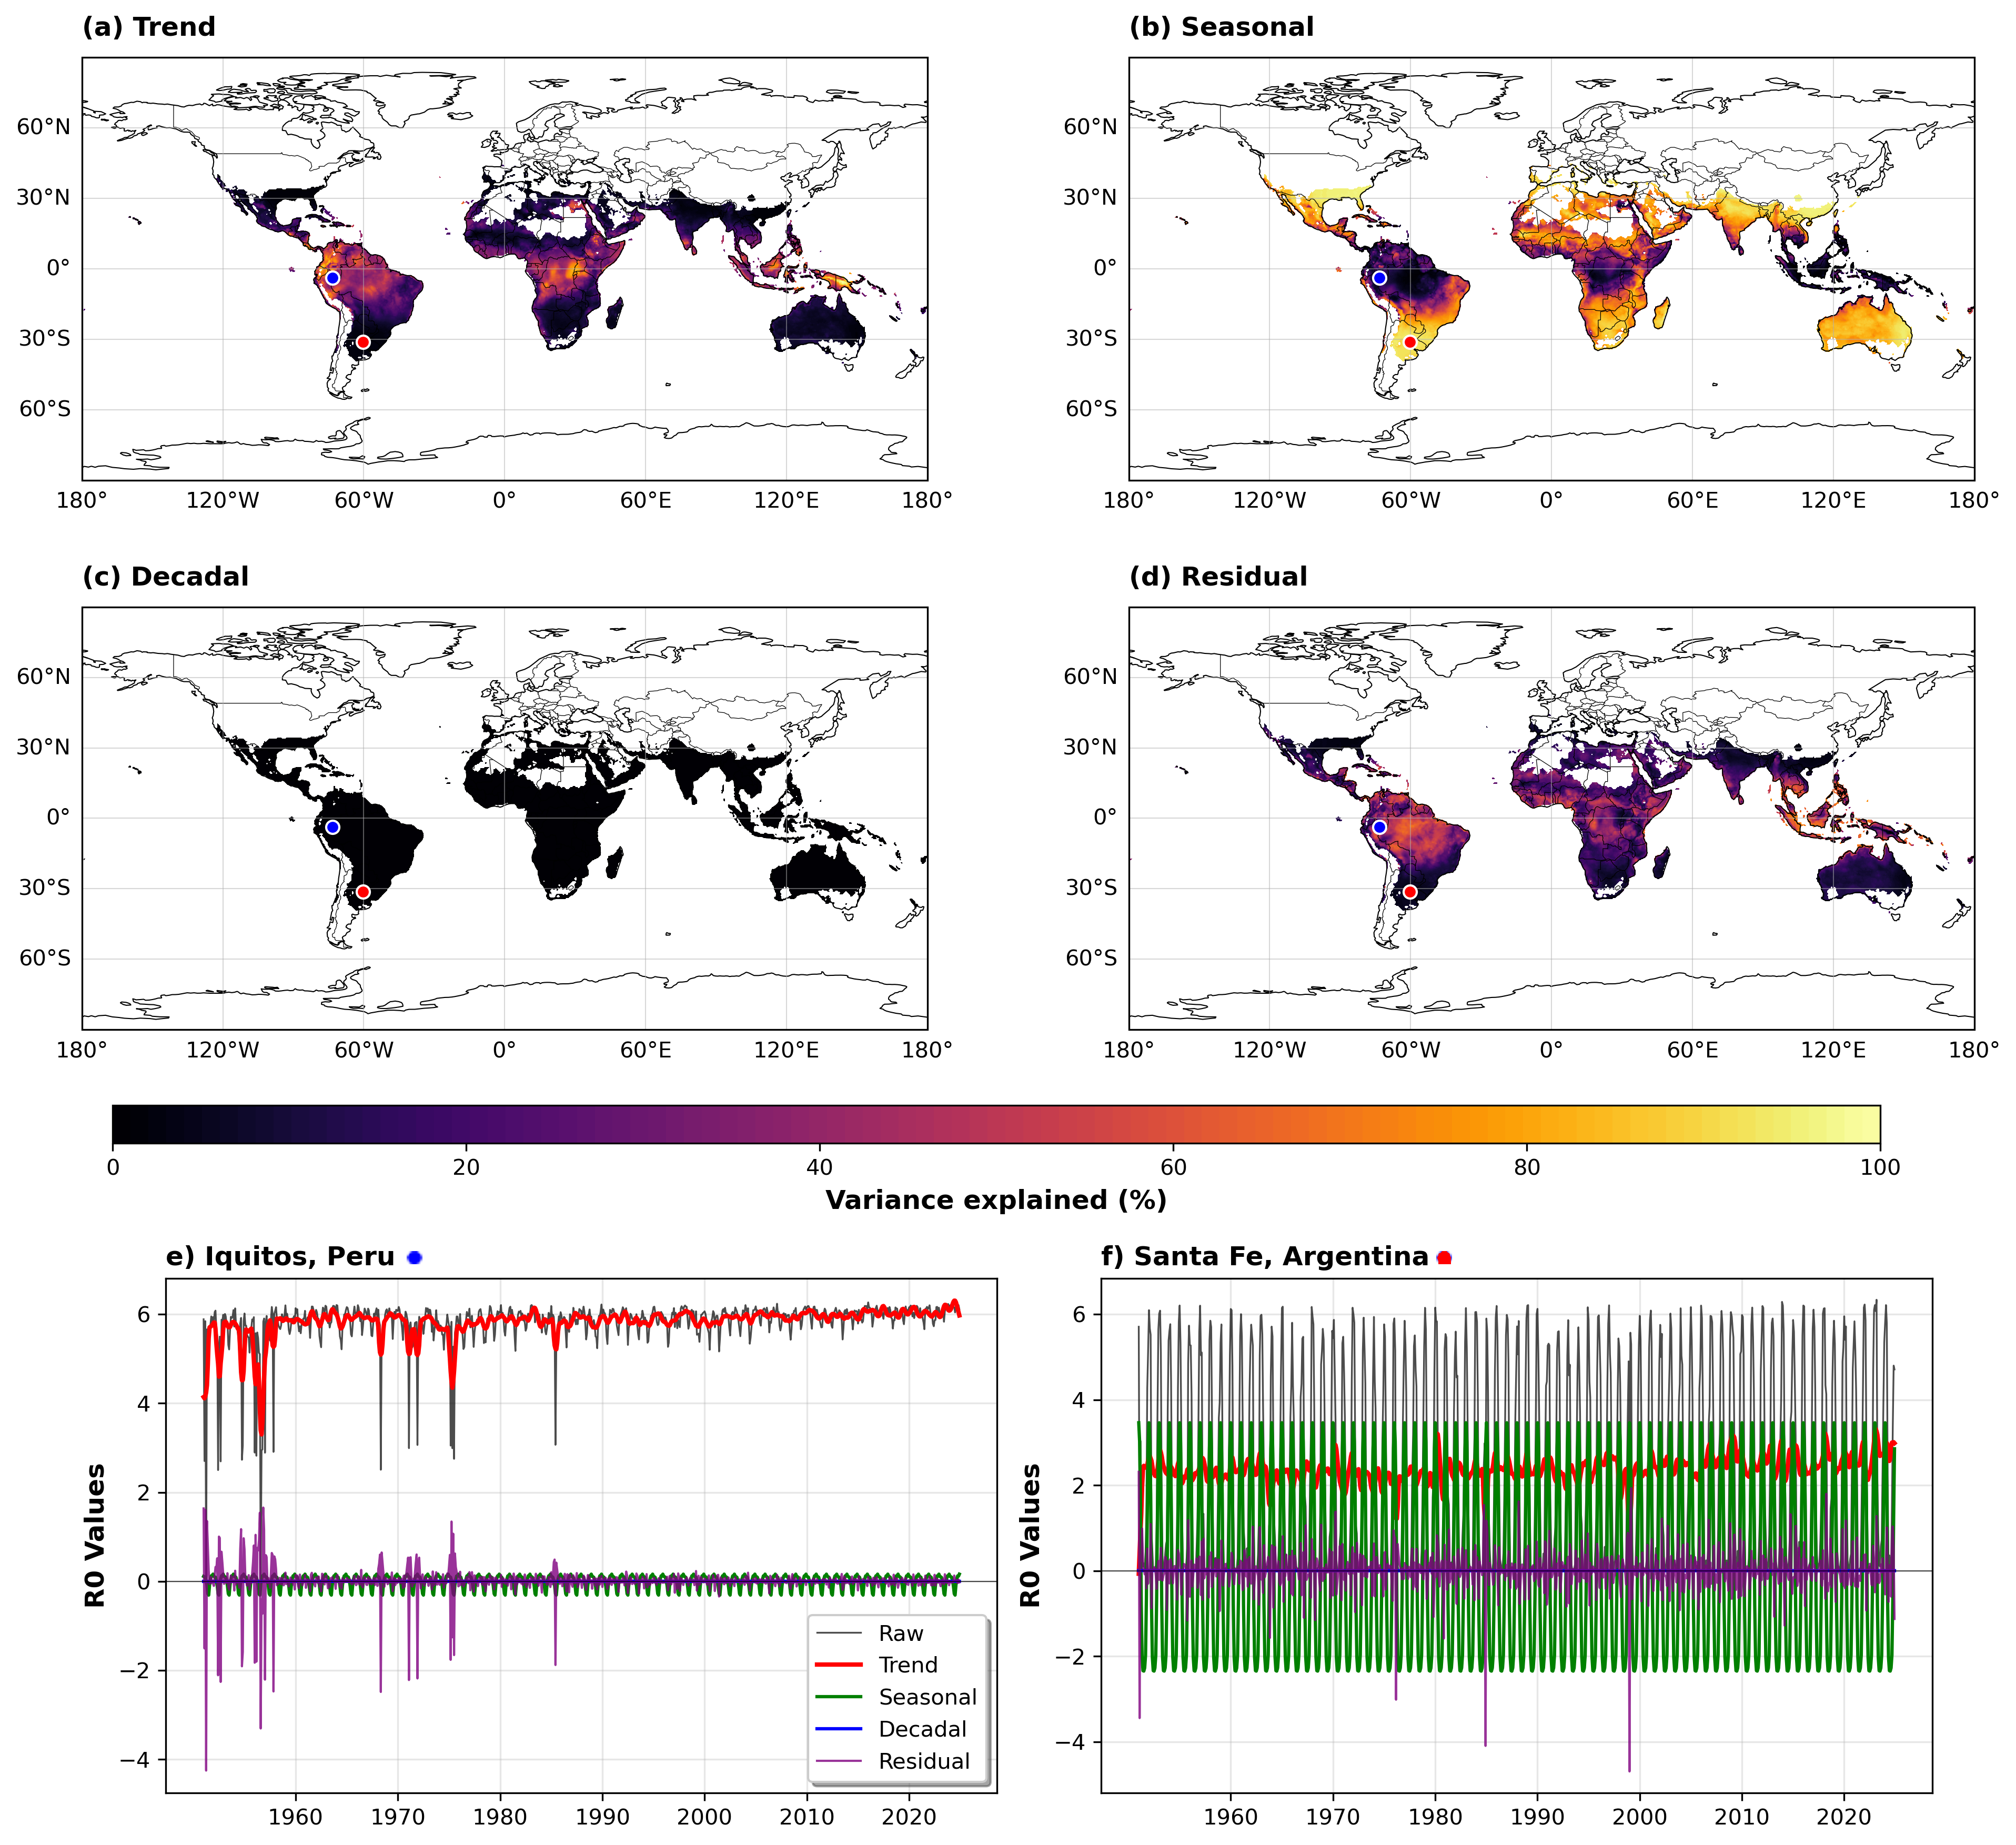
\includegraphics[width=\textwidth]{timescale_decomposition_combined_ps.png}
  \caption{\textbf{a)-d)} Global timescale decomposition maps for $R_0$ values for the monthly mean 1951-2024 period, different components. The time series for the cities of Iquitos, Peru (blue dot), and Santa Fe, Argentina (red dot), are shown as examples in \textbf{e)} and \textbf{f)} respectively.}
  \label{fig:global-timescale-decomposition}
\end{figure*}
\begin{figure*}[!ht]
  \centering
  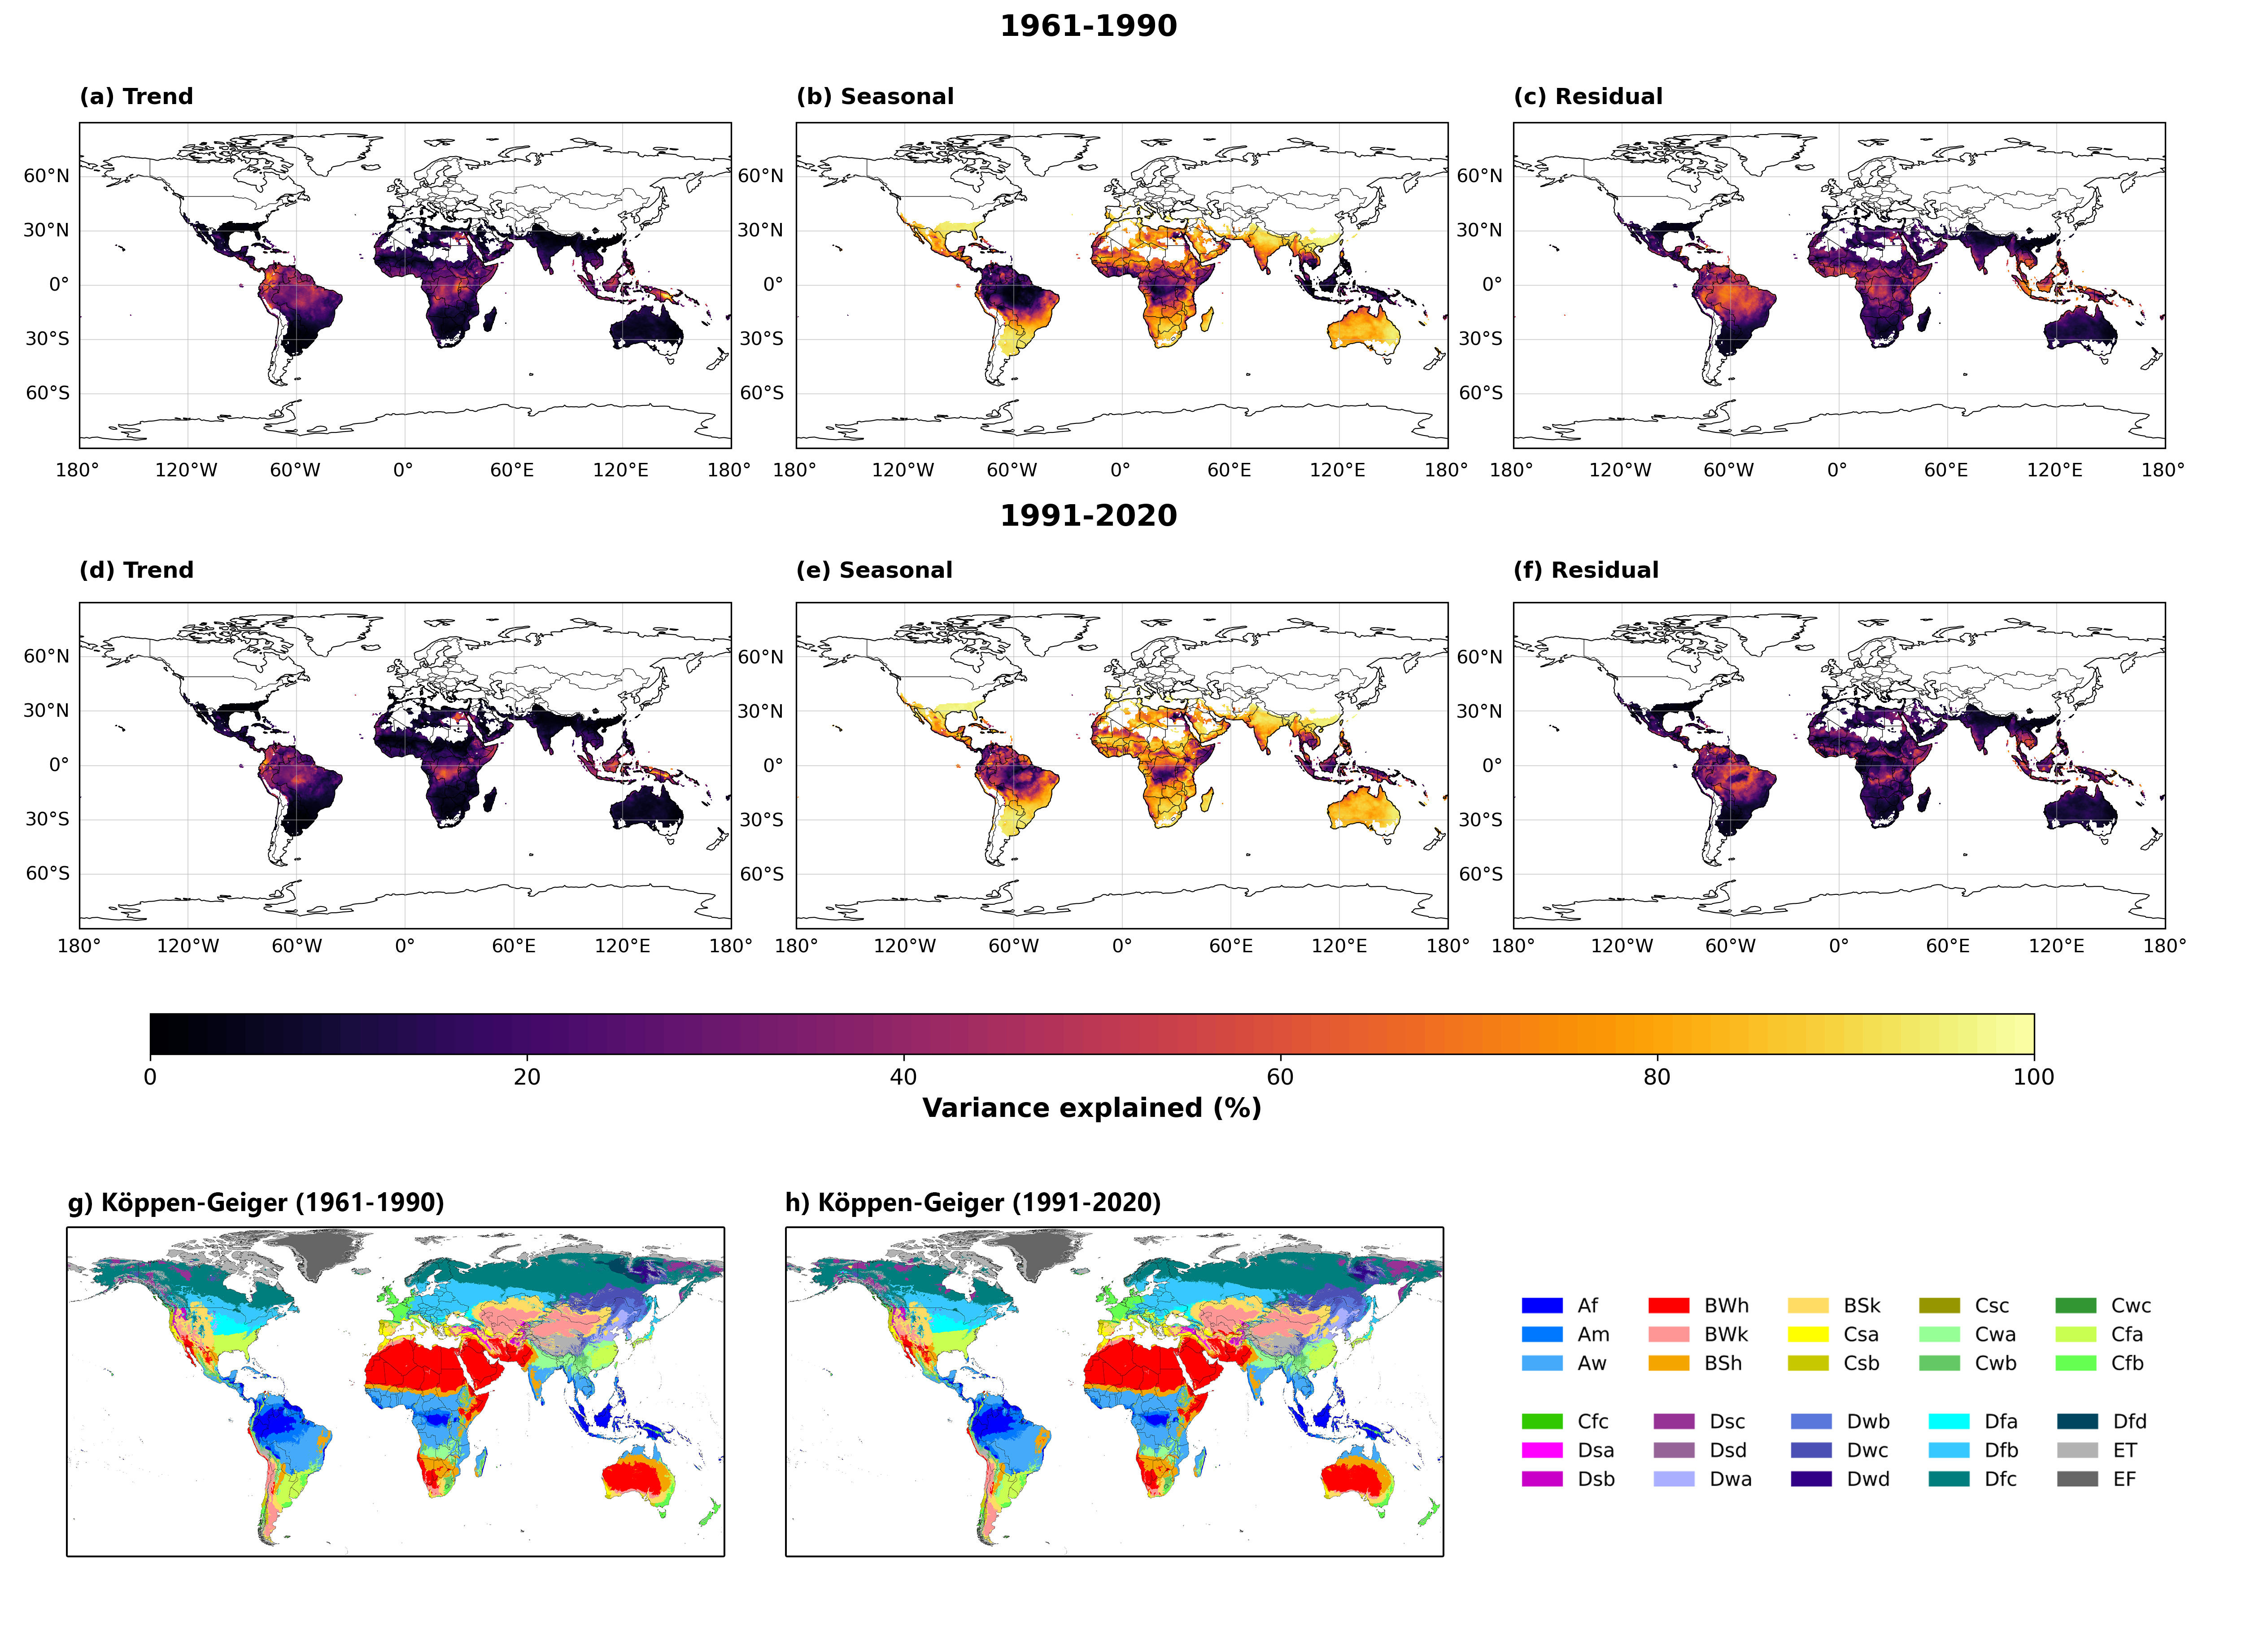
\includegraphics[width=\textwidth]{timescale_decomposition_climatology_comparison_ps.png}
  \caption{\textbf{a)-c)} Global timescale decomposition maps for $R_0$ values for the monthly mean 1961-1990 period, different components. Its associated Köppen-Geiger climate classification is shown in \textbf{g)}. \textbf{d)-f)} Global timescale decomposition maps for $R_0$ values for the monthly mean 1991-2020 period, different components. Its associated Köppen-Geiger climate classification is shown in \textbf{h)}. (Source for Köppen-Geiger climate classification maps: \cite{beck_2023})}
  \label{fig:global-timescale-decomposition-2}
\end{figure*}

The resulting timescale decomposition maps for $R_0$ global outputs for the whole time series can be found in Figure \ref{fig:global-timescale-decomposition}, along with the component time series for the cities of Iquitos, Peru, known to be a traditional hotspot of \textit{Aedes}-borne diseases, and Santa Fe, Argentina. The optimal span values of LOESS smoothing for the timescale decomposition methodology for this sample period were found to be 5, 7 and 8 months for the $R^2$, $AIC$ and $GCV$ verification metrics respectively, with the GCV-associated value being selected out of the three due to the aforementioned reasons explained in Section \ref{sec-methods-1-methodology}. It is worth noting that, because the $R_0$ metric operates in certain temperature ranges, grid points with less than 6 months of data per year were excluded from the analysis, in order to prevent poor seasonal component estimation due to missing entire seasons.
\\
\\
Over the 74-year period, the long-term trends and residual components of $R_0$ (Figures \ref{fig:global-timescale-decomposition}a and \ref{fig:global-timescale-decomposition}d) show the highest variance contribution in tropical and subtropical regions, particularly across central Africa, parts of South America including the Amazon basin, and scattered areas in Southeast Asia and northern Australia (the sum of these components rounding between 40-80\%). These trend patterns suggest that long-term climate change, along with interannual climate variability, is driving systematic shifts in $R_0$ in these traditionally endemic regions, reflecting the complex interactions between temperature, humidity, and precipitation influencing vector populations and virus transmission. For these regions, there is no clearly defined transmission season over the year, as the seasonal signal of $R_0$ (Figure \ref{fig:global-timescale-decomposition}b and \ref{fig:global-timescale-decomposition}e) is rather poor. Instead, the climatology of $R_0$ in these regions, due to the high temperature and humidity values, adopts high $R_0$ values which remain constant throughout the year, independently of the season.
\\
\\
Though the decadal component (Figure \ref{fig:global-timescale-decomposition}c) shows a nigh negligible contribution across all regions of the globe, the seasonal variance (<5\%, Figure \ref{fig:global-timescale-decomposition}b) shows a markedly different geographical distribution, with the highest contributions (between 60-100\% variance explained) concentrated in regions with pronounced seasonal temperature variations. Notable hotspots include the northern edges of traditional dengue transmission zones in South America, parts of southern Africa, central Asia, and importantly, temperate regions that border current endemic areas. It is in these regions where the seasonal temperature fluctuations strongly condition the transmissibility season of $R_0$, reaching its peak around the summer months.
\\
\\
Indeed, Figure \ref{fig:global-timescale-decomposition}(f) highlights the effect of the seasonal component on the overall $R_0$ dynamics in these strong seasonal regions. While the trend component accounts for a significant portion of the variance, it is the seasonal component that can play a crucial role in defining whether a DENV outbreak can occur ($R_0$ > 1) or not ($R_0$ < 1).
\\
\\
Two subsets of the seasonal variance results, corresponding to the 1961-1990 and 1991-2020 climatologies, can be found in Figure \ref{fig:global-timescale-decomposition-2}, along with their respective Köppen-Geiger climate classification maps\cite{beck_2023}. For these two periods, the GCV-optimal span value of LOESS smoothing is also 8 months, same as for the complete time series.
\\
\\
When examining the variance patterns in relation to the Köppen-Geiger classification, distinct climate zone signatures can become apparent on a first-approximation basis. Tropical climate zones (A-type climates in the Amazon basin, central Africa, and Southeast Asia) demonstrate characteristic patterns where trend and residual variance typically dominates. Alternatively, temperate and humid subtropical zones (C-type climates in southern Brazil, parts of East Asia, and the Mediterranean basin) show a more pronounced seasonal component. At a glance, it may seem that a study on the expansion of A and C type Köppen Geiger climates in the context of climate change may provide a useful framework for predicting the evolution of \textit{Aedes}-borne transmissibility, with each major climate type exhibiting distinct characteristics that condition the $R_0$ signal.
\\
\\
However, this would be a naive approach, since the Köppen-Geiger classification is a static classification system that does not thoroughly reflect the dynamic nature of climate change\cite{triantafyllou_1994}. Indeed, the comparison between the two 30-year periods reveals notable shifts in how climate variability affects $R_0$ across different regions. In the 1961-1990 period, the trend component shows more concentrated high-variance zones, particularly in central Africa and tropical parts of South America. By the later 1991-2020 period, these trend patterns have intensified in some regions while diminishing in others, highlighting that the impacts of systematic climate change on transmission potential, while shown to have become more pronounced over time, are not entirely straightforward.
\\
\\
Given the strong seasonality of $R_0$ in temperate regions through these timescale decomposition analyses, and given the different climate variables that \textit{Aedes}-borne transmissibility seems to relate to besides temperature, it is not unreasonable to expect $R_0$ values to be closely related to seasonal, temperature-driven climate patterns, be it in the form of correlation or causality. The following analyses aim to explore these relationships further, with the climate variability indices previously listed in Table \ref{tab:climate-variability-indices}.

\subsection{Analysis 2: Correlation studies between $R_0$ and climate variability indices} \label{sec-results-2} \label{sec-results-2}

\begin{figure*}[!ht]
  \centering
  \includegraphics[width=\textwidth]{correlation_seasonal_global_niño_34_ps.png}
  \caption{\textbf{a)-d)} Correlation values between $R_0$ and the Niño 3.4 index, for the 1951-2024 monthly mean period in all seasons. Dots represent statistically significant correlation values, at $p < 0.01$.}
  \label{fig:global-correlation-niño-34}
\end{figure*}

\begin{figure*}[!ht]
  \centering
  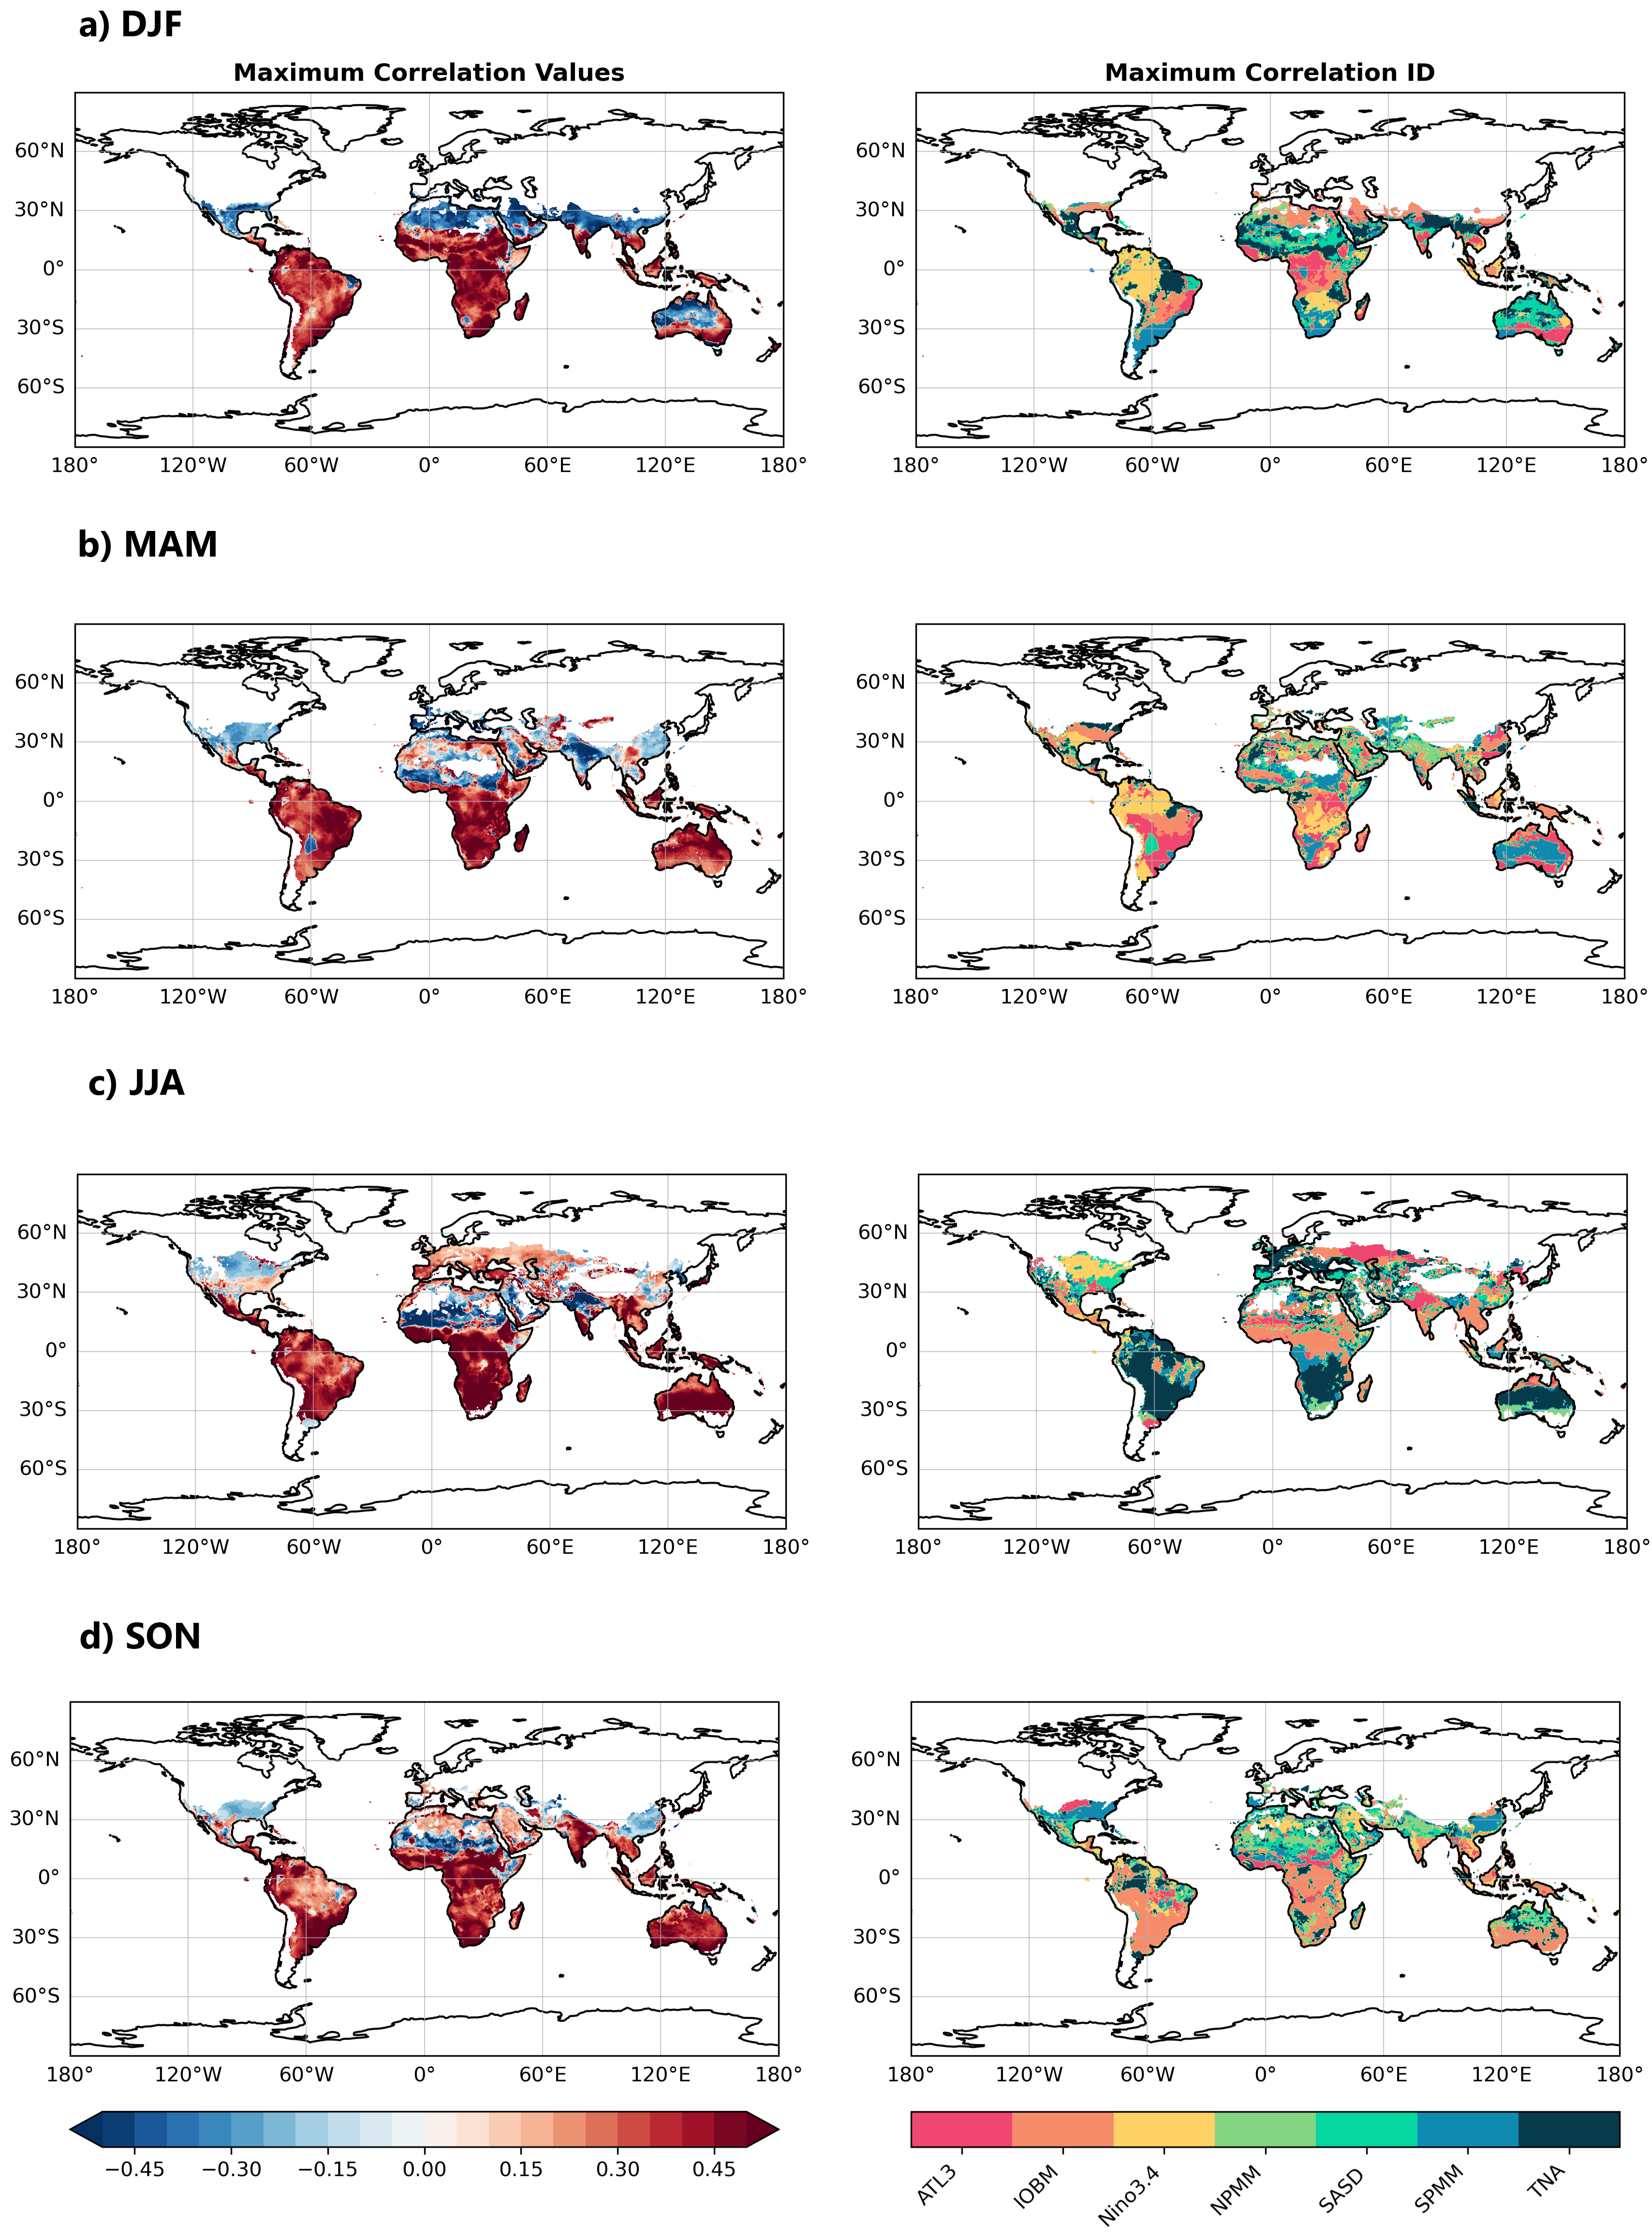
\includegraphics[width=0.9\textwidth]{correlation_final_global_ps.png}
  \caption{\textbf{a)-d)} For all seasons: Left, maximum statistically significant correlation values between $R_0$ and all indexes of Table \ref{tab:climate-variability-indices}, for the 1951-2024 monthly mean period. Right, which climate index gives the maximum statistically significant correlation values.}
  \label{fig:global-correlation-final}
\end{figure*}

\begin{figure*}[!ht]
  \centering
  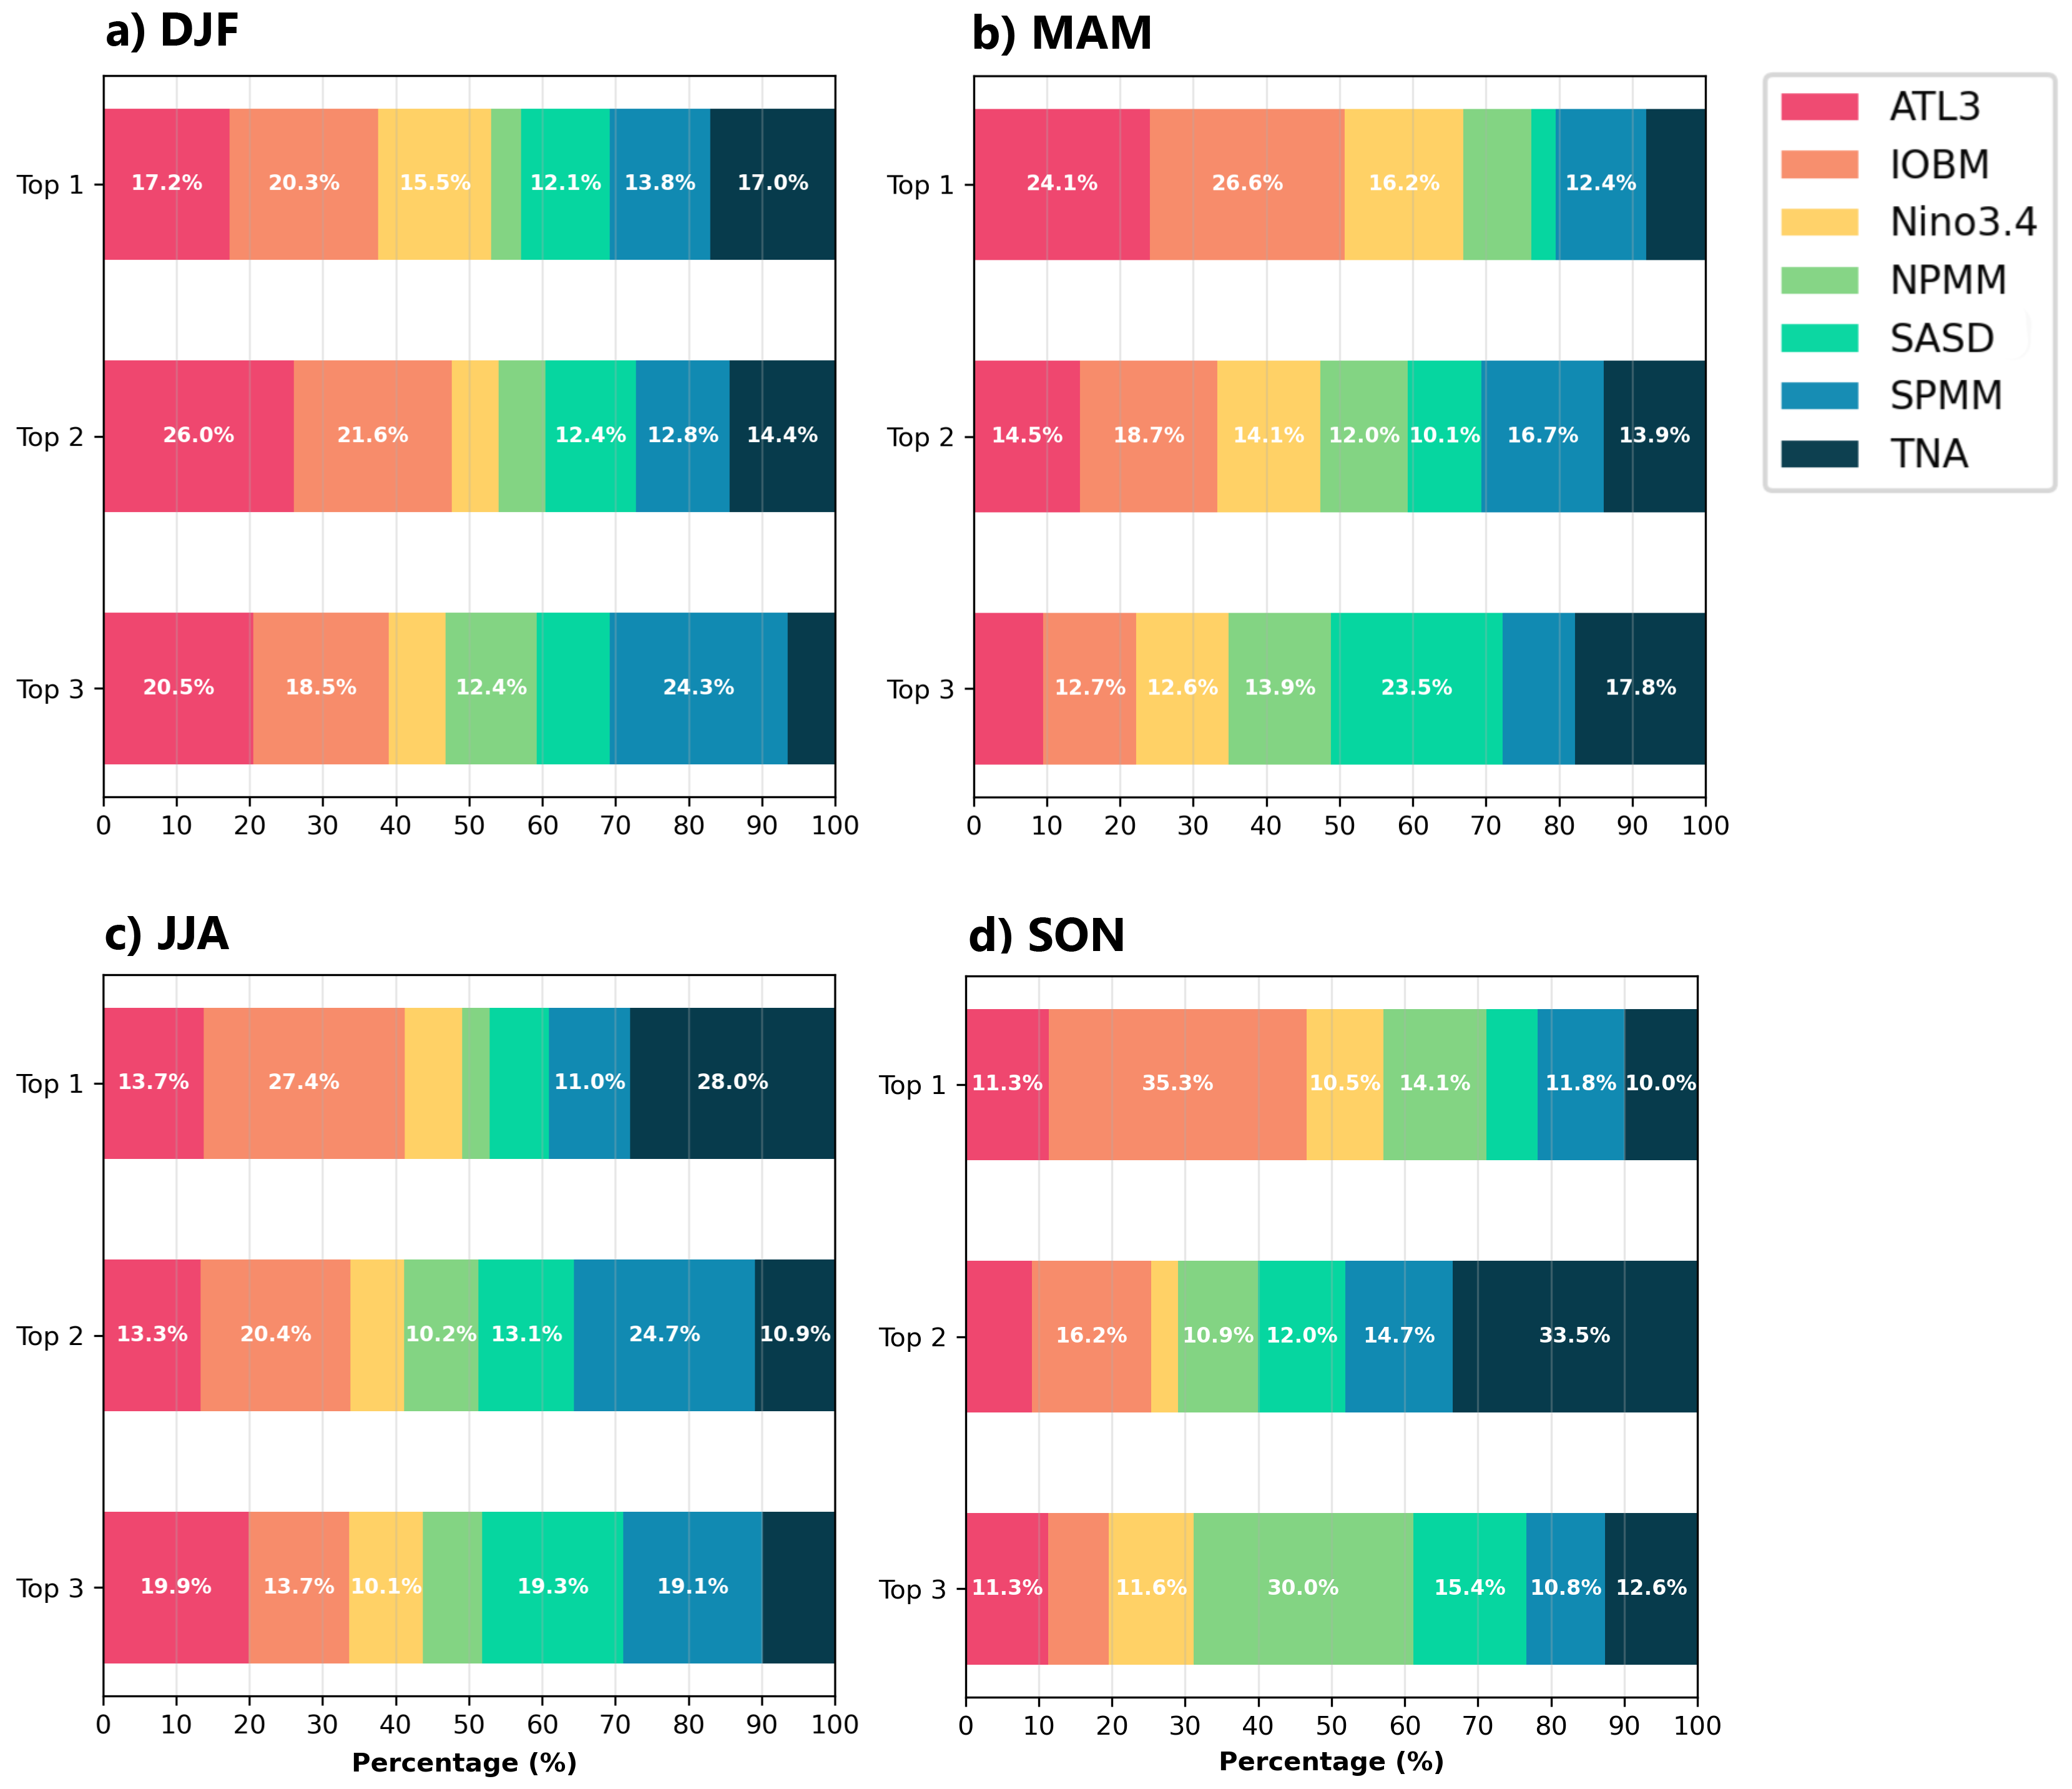
\includegraphics[width=0.75\textwidth]{correlation_barplots.png}
  \caption{\textbf{a)-d)} For all seasons: Percentage of grid points over which each index gives the highest, second or third highest statistically significant causality values.}
  \label{fig:panama-correlation-niño-34}
\end{figure*}

\begin{figure*}[!ht]
  \centering
  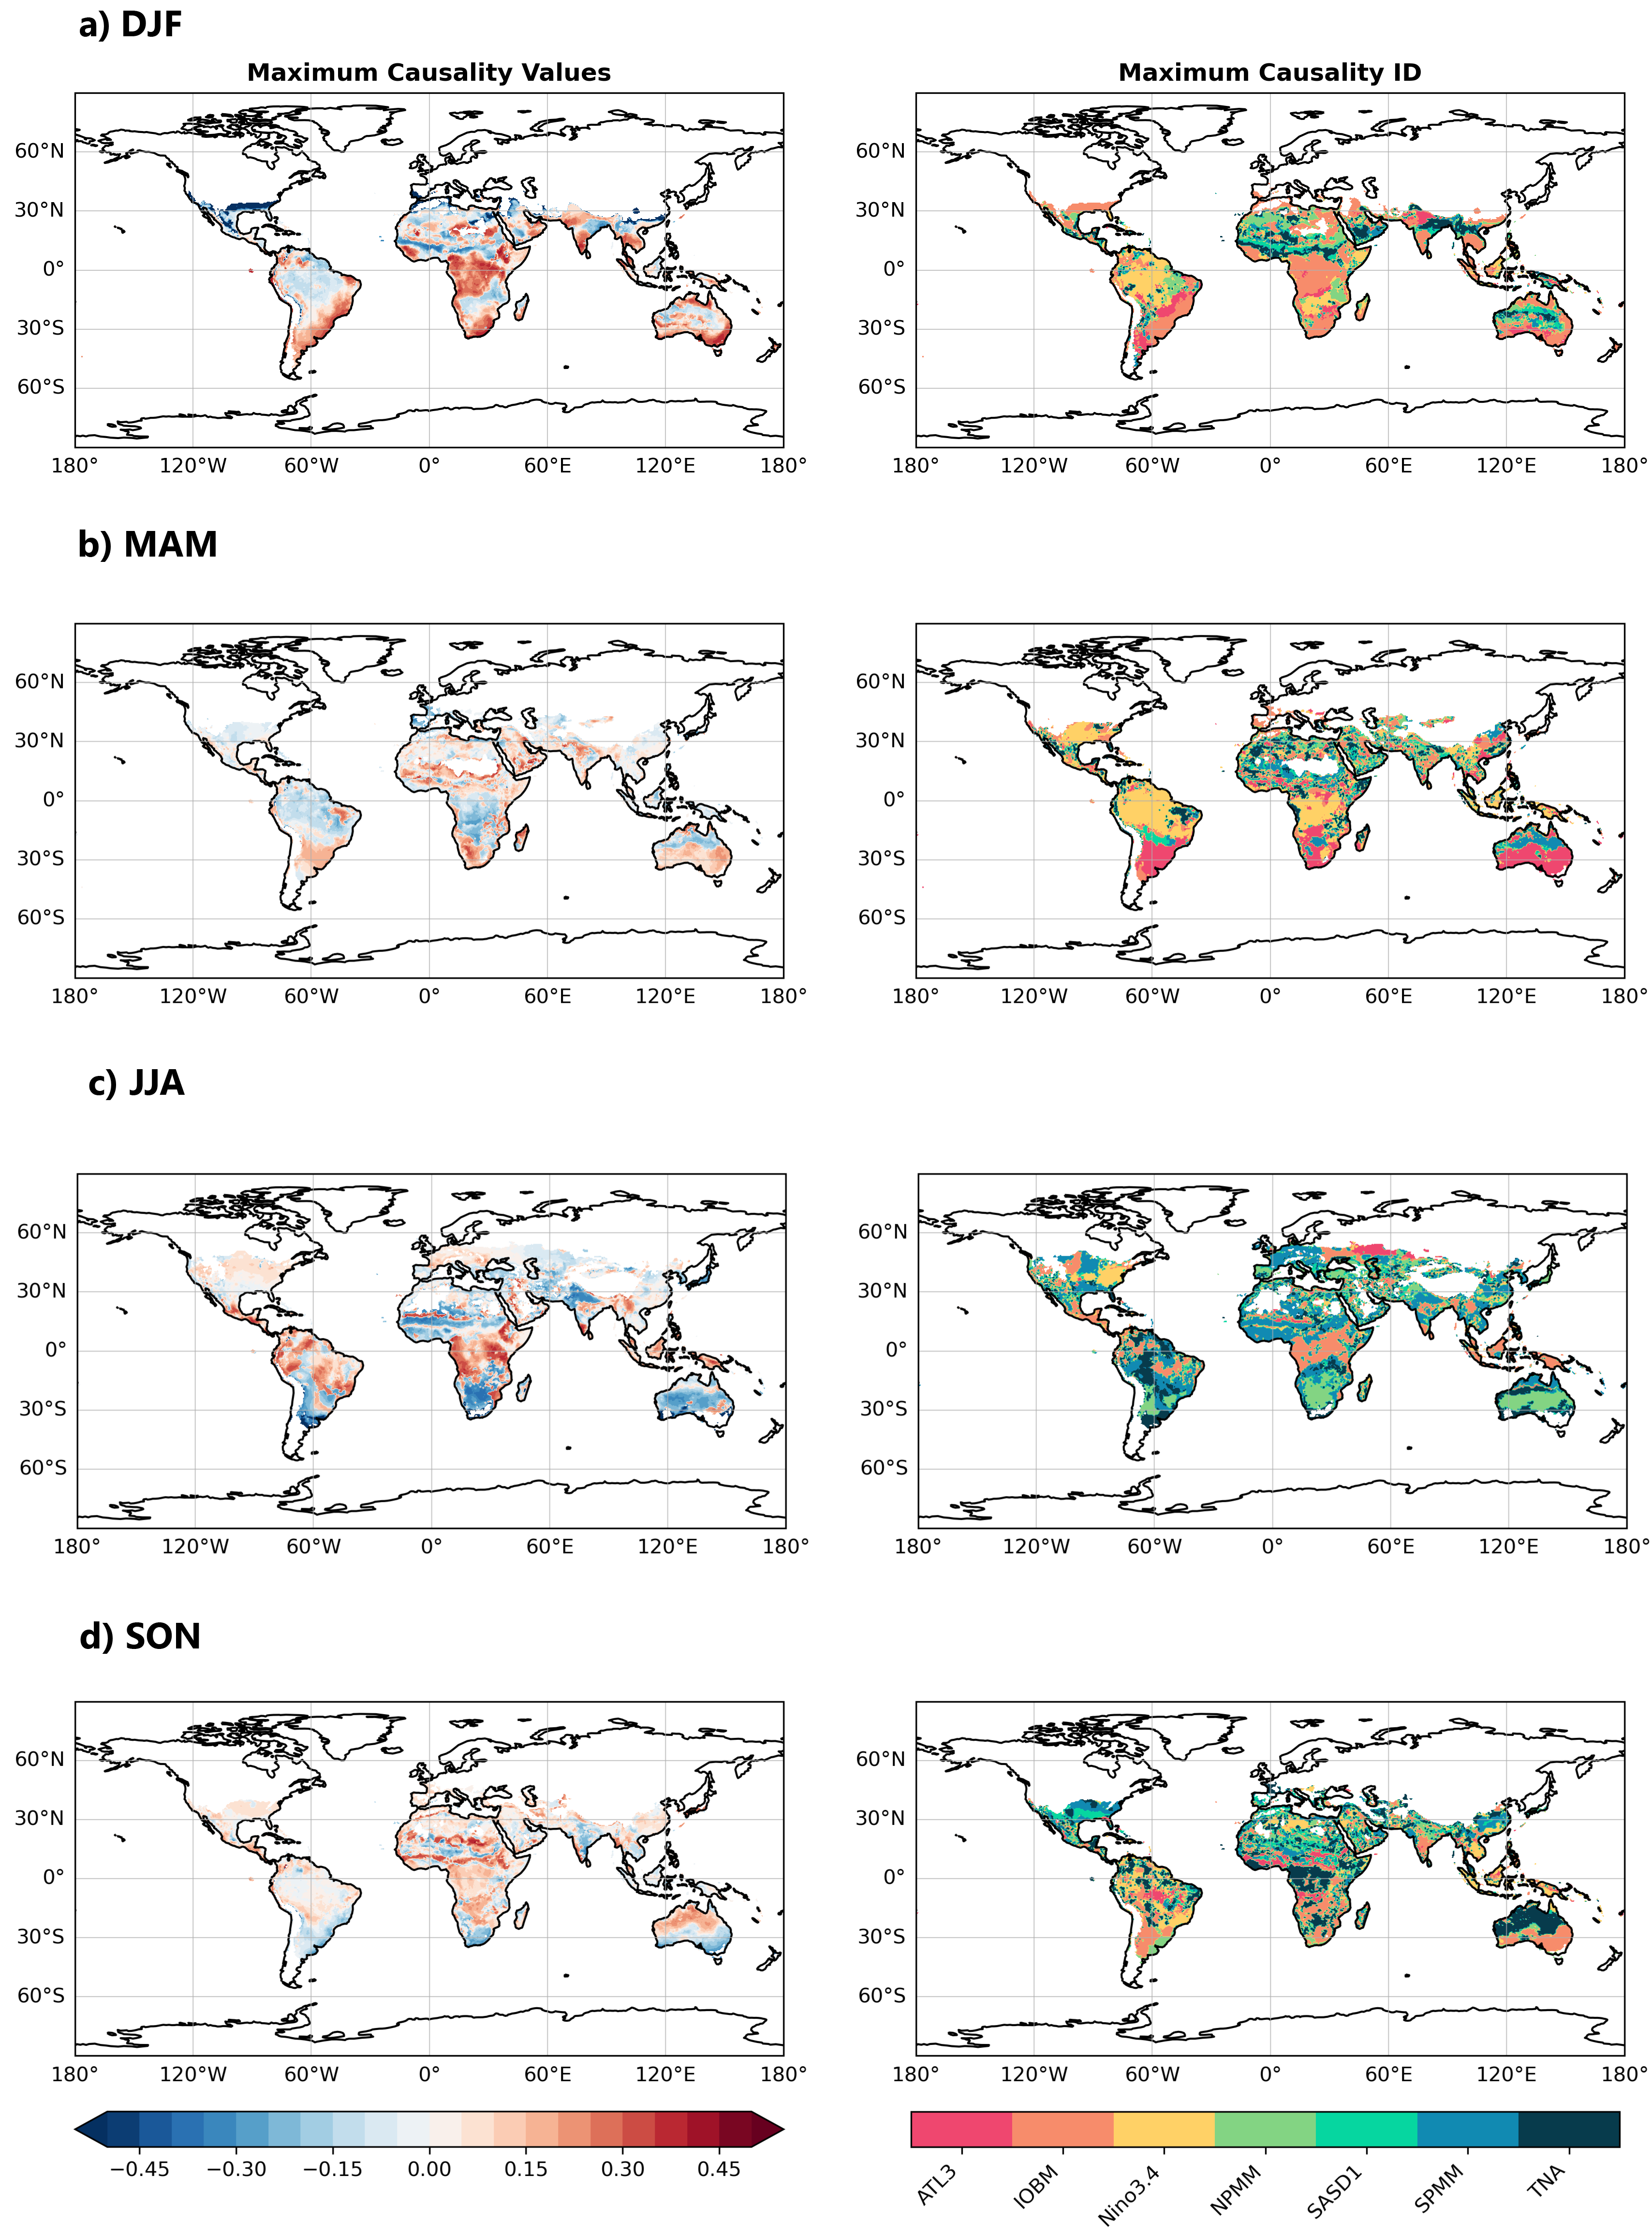
\includegraphics[width=\textwidth]{causality_final_global_ps.png}
  \caption{\textbf{a)-d)} For all seasons: Left, maximum statistically significant causality values between $R_0$ and all indexes of Table \ref{tab:climate-variability-indices}, for the 1951-2024 monthly mean period. Right, which index gives the maximum statistically significant causality values. }
  \label{fig:global-causality-final}
\end{figure*}

\begin{figure*}[!ht]
  \centering
  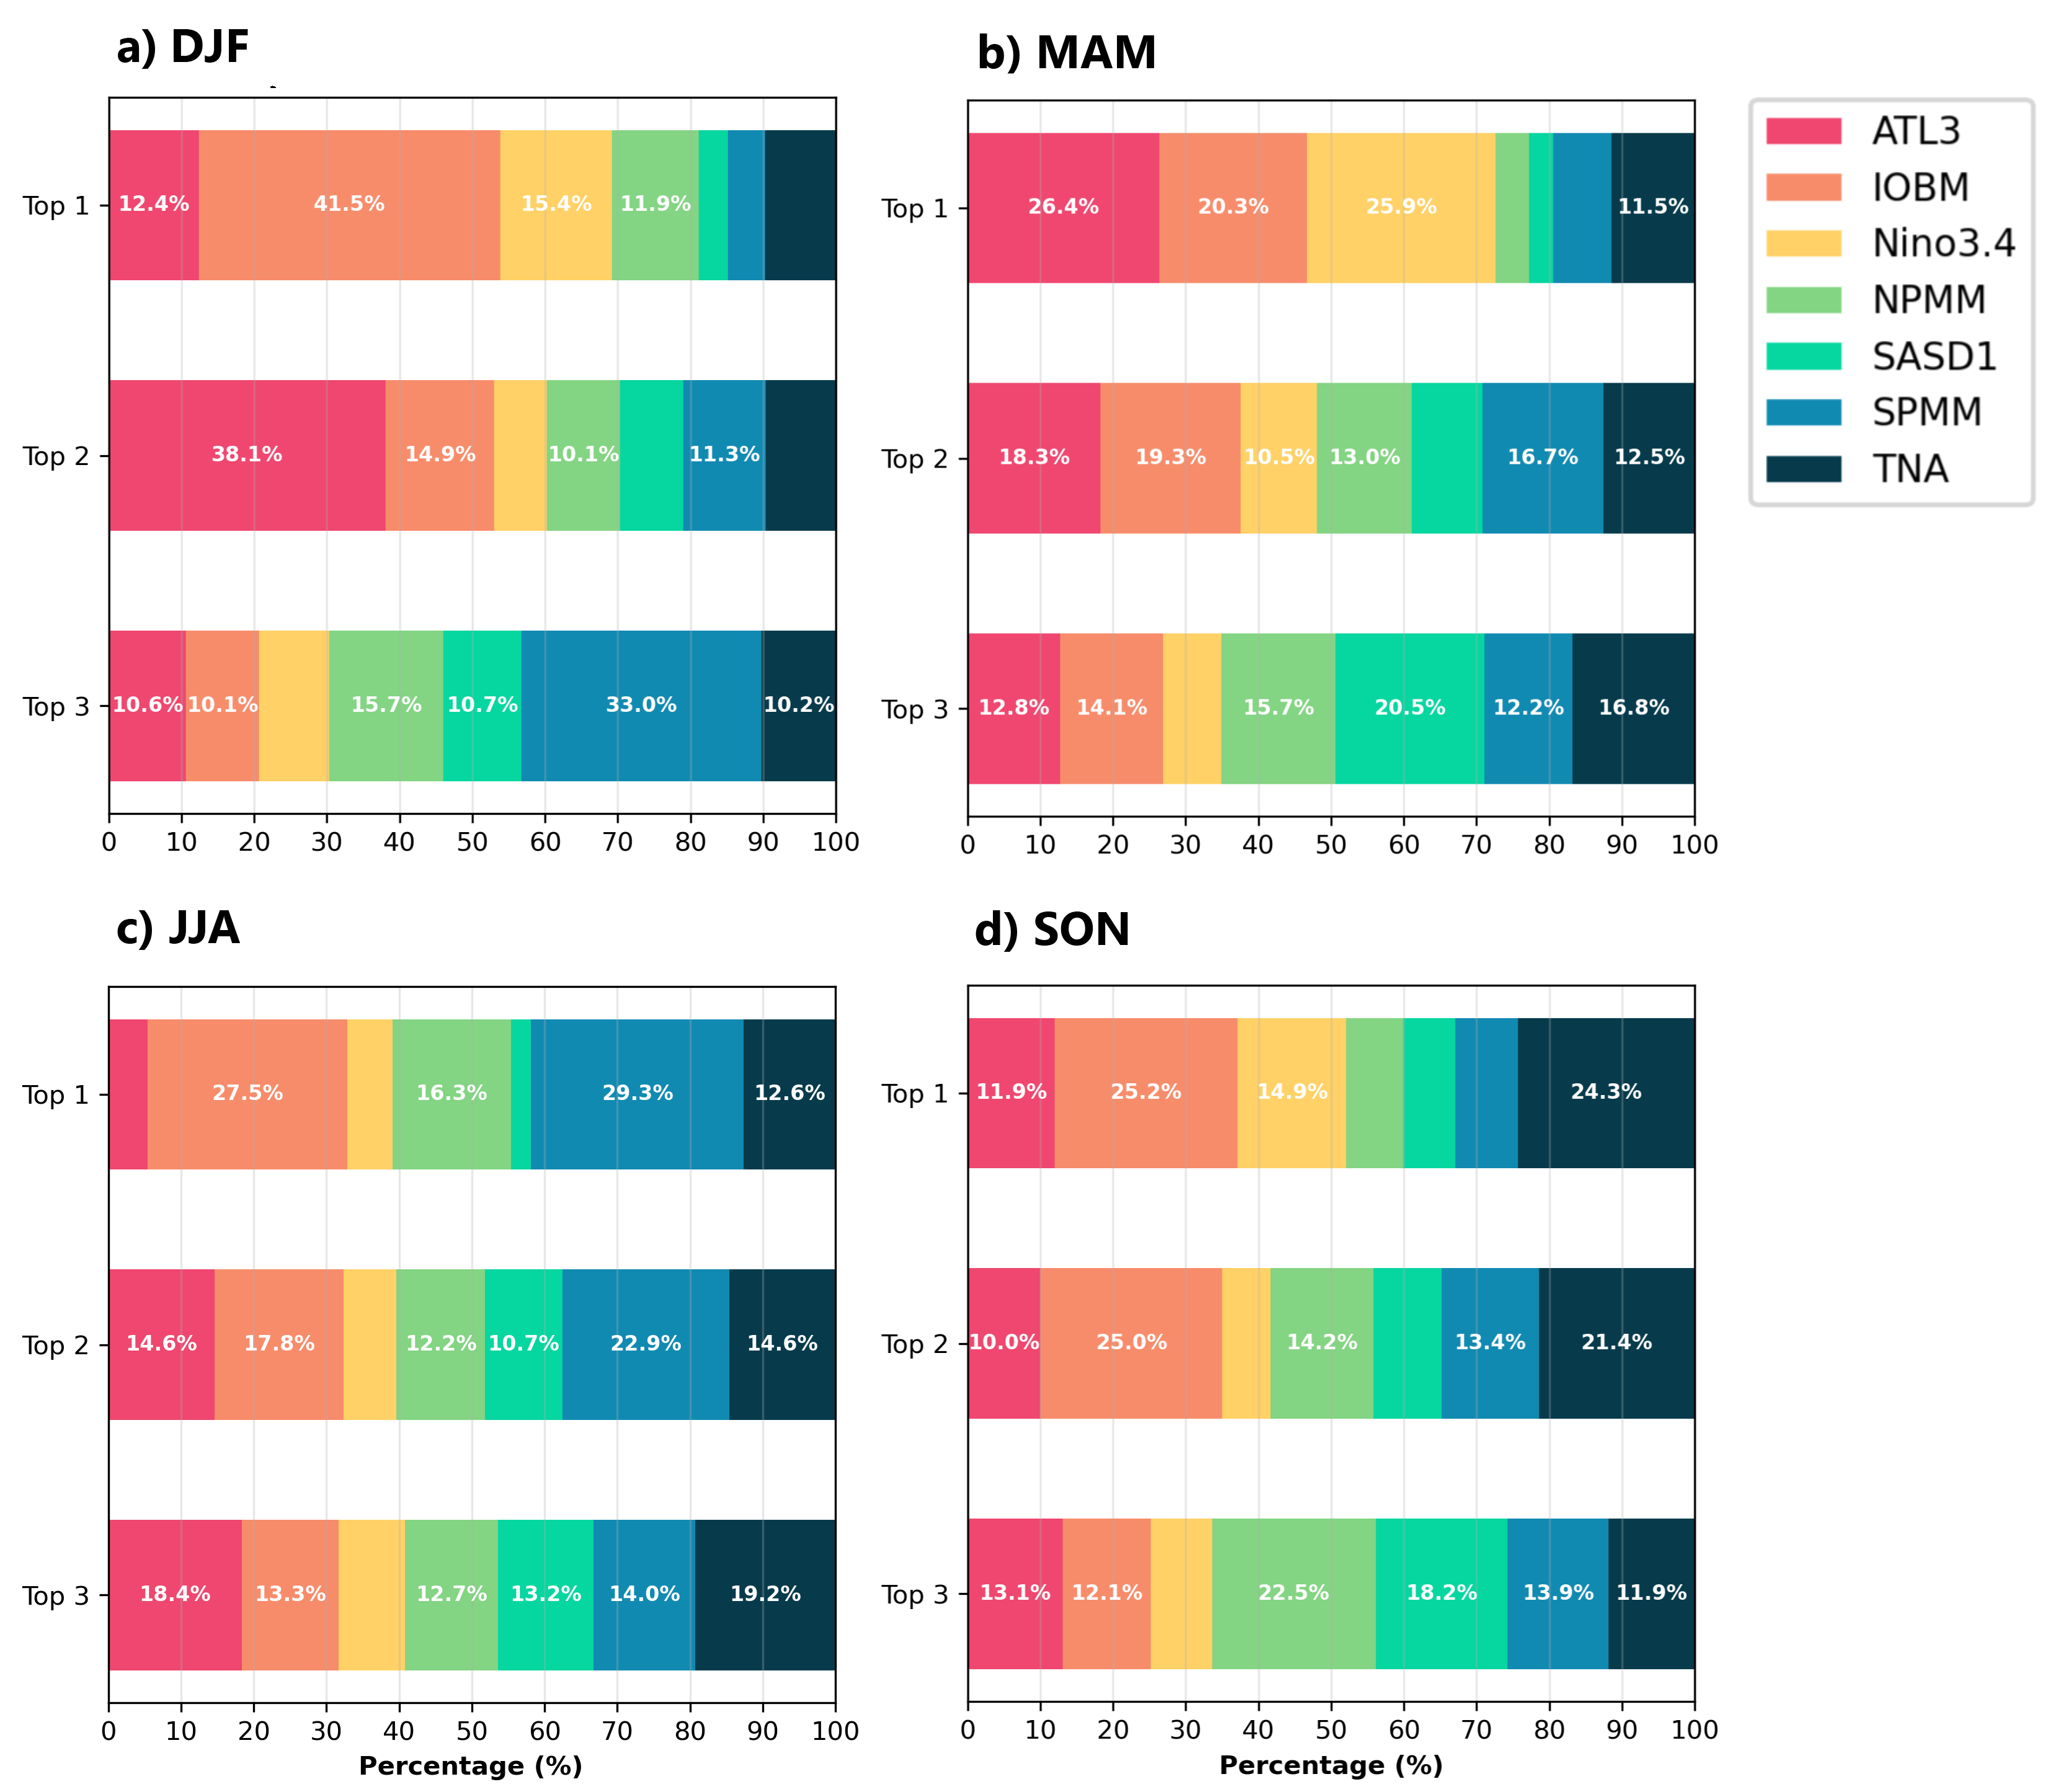
\includegraphics[width=0.75\textwidth]{causality_barplots.png}
  \caption{\textbf{a)-d)} For all seasons: Percentage of grid points over which each index gives the highest, second or third highest statistically significant causality values.}
  \label{fig:panama-causality-barplots}
\end{figure*}

\subsection{Analysis 3: Causality studies between $R_0$ and climate variability indices. Outlining of predictors for disease outbreaks} \label{sec-results-3}

\section{Discussion} \label{sec-discussion}

\subsection{The added value of climate patterns in seasonal forecasting of \textit{Aedes}-borne diseases} \label{sec-discussion-added-value}

\subsection{Analysis 1: Multi-timescale climate decomposition of $R_0$} \label{sec-discussion-analysis-1}

\subsection{Analyses 2 and 3: Correlation and causality studies between $R_0$ and climate variability indices} \label{sec-discussion-analysis-2-3}

\subsection{Notable limitations and constraints} \label{sec-discussion-limitations}

\section{Conclusions} \label{sec-conclusions}

\begin{enumerate}
  \item Historical and climatological analyses of $R_0$ values for \textit{Aedes}-borne diseases provide insight in understanding the role of climate in disease emergence, and can be used to improve the accuracy of seasonal forecasts through the identification of climate predictors. However, while global climate models are suitable for a broad, general-purpose understanding, high-resolution data is preferred when more nuanced analysis are performed in endemic regions, in order to provide more accurate and actionable information for public health officials.
  \item
\end{enumerate}

\section{Additional files} \label{sec-additional-files}

\section{Abbreviations} \label{sec-abbreviations}
\begin{itemize}
  \item AeDES2: \textit{Ae}des \textit{D}isease \textit{E}nvironmental \textit{S}uitability 2
  \item AIC: Akaike Information Criterion
  \item ATL3: Atlantic 3 Index
  \item CHIKV: Chikungunya
  \item DENV: Dengue
  \item ENSO: El Niño Southern Oscillation
  \item GCV: Generalized cross-validation
  \item IOB: Indian Ocean Basin
  \item IOD: Indian Ocean Dipole
  \item LOESS: Locally estimated scatterplot smoothing
  \item NPMM: North Pacific Meridional Mode
  \item $R^2$: Coefficient of determination
  \item SASD: South Atlantic Subtropical Dipole
  \item SIOD: Southern Indian Ocean Dipole
  \item SPMM: South Pacific Meridional Mode
  \item TNA: Tropical North Atlantic
  \item VBDs: Vector-borne diseases
  \item WHO: World Health Organization
  \item ZIKV: Zika
\end{itemize}

\section{Acknowledgements} \label{sec-acknowledgements}

\section{Funding} \label{sec-funding}

\section{Availability of data and materials} \label{sec-availability}
Code for the generation of $R_0$ values employed for this study, computed using AeDES2's monitoring system, is available under request, and its values can be visualized in an operational, in-development Shiny App (link) for any region and grid-point. Additionally, the necessary datasets, functions and scripts to generate the maps and plots for this manuscript and supplementary material are available under the following GitHub repository: \url{https://github.com/jacorvillo/monitoring_system_analysis}

\section{Authors' contributions} \label{sec-authors-contributions}

Á.M., V.T. and D.C. conceived the methodology to be undertaken in this manuscript. Data sources, code and figures were obtained and developed from the ground up by J.C, who also analysed the results. All authors have reviewed the manuscript.

\section{Ethics approval and consent to participate} \label{sec-ethics-approval}
Not applicable.

\section{Consent for publication} \label{sec-consent-for-publication}
Not applicable.

\section{Competing interests} \label{sec-competing-interests}
The authors declare no competing interests.

\section{Author details} \label{sec-author-details}

\section{References} \label{sec-references}

\bibliography{references}

\end{document}